\documentclass[conference]{IEEEtran}

%%%%% PREAMBLE

% Global document settings
\usepackage[T1]{fontenc}			% to adjust fonts to language type
\usepackage[utf8]{inputenc}		% to apply UTF-8 encoding
\usepackage[nolist]{acronym}
\usepackage{algorithmic}
\algsetup{
	linenosize=\small,
}
\usepackage{amsmath}
\usepackage{graphicx}
\usepackage{booktabs}

% This document settings
\title{An audio lossy codec with\\ Vector Quantization (VQ)}
\author{\IEEEauthorblockN{João Fonseca, Pedro Silva and Rui Lopes}
\IEEEauthorblockA{Departamento de Eletrónica, \\
Telecomunicações e Informática\\
Universidade de Aveiro, Portugal\\
Email: \{jpedrofonseca,pedro.mfsilva,ruieduardo.fa.lopes\}@ua.pt}}

%%%%% END PREAMBLE

%%%%% DOCUMENT 

\begin{document}

\begin{acronym}
	\acro{LBG}[LBG]{Linde-Buzo-Gray}
	\acro{PCM}[PCM]{pulse-code modulation}
	\acro{WAV}[WAV]{waveform audio file format}
	\acro{dB}[dB]{decibel}
\end{acronym}

\maketitle

%%% Abstract
\begin{abstract}
	Nowadays most of the audio service providers such as Apple Music, Pandora Radio or Spotify distribute their content seamlessly throughout the Internet. This happens due to the power of compression, where a large array of versions of each user requested music track is compressed at a different sample bit length, most of them being made lossy codecs. As lossy codecs are made to exclude data from an audio file which could be identified as redundant, this work shows a construction of a lossy audio codec, based on Vector Quantization (VQ).
\end{abstract}

%%% Keywords
\begin{IEEEkeywords}
	audio codec, compression, lossy compression, vector quantization	, VQ
\end{IEEEkeywords}

%%% FIRST SECTION - Introduction
\section{Introduction}

In most recent years, the amount of music applications used by people in general has been increasing exponentially, due to both lower costs in accessing the contents, and the low delays on the service capabilities of its distribution.

This distribution of audio content can be attained in such a small delay transport since its transmission counts with the help of an advance made back in the history of computing and of information: the compression. In fact, most of today's audio services like Apple Music, Pandora or Spotify use compression to reduce the amount of redundant and dispensable data in audio tracks. The user, unable to distinguish the differences, receives a smaller version of the original record, easing its transmission throughout the networks.

This document relates to the design and the implementation of an audio codec classified as \textit{lossy}, that is, which dispensable and redundant data is lost by the means of compression, and which compressed format is not audible. Some tools were also made in order to evaluate the development of the audio codec, also hereby described.

%%% SECOND SECTION - Architecture
\section{System Architecture}

This audio codec is designed to perform compression throughout a mechanism of quantization. In fact, as soon as the input is given to our system, a first module would apply \emph{uniform quantization} to it. This way, given an audio as an input (audio file in \ac{WAV})  and in 16-bits \ac{PCM} format), it is expected this first module tries to remove some of the least significant bits of the samples representation—with this method some of the audio contents are replaced with noise artifacts, nonetheless the media remains audible and understandable to most people.

After this first modification, which would have as an output a \texttt{\acs{WAV}} file with reduced samples (in content, not in length, since we have to restore the original 16-bit samples in order to reproduce the audio on a conventional player), each of these must be given into a module which would reproduce a \emph{codebook}, that is, a set of codewords that allows this module to replace a uniformly quantized sample into the representation of the closest vector within itself. Basically, this module is a bi-dimensional vector with $c$ codewords of $b$ bits, made having in mind the audio object to compress. The representation which will then replace the sample on the compressed file, is the index of the codeword vector which was evaluated to be the closest one in comparison with the given sample.

These described modules would be applied by an entry-point which would also have an encoder and decoder components. The \emph{encoder} would have the function to apply the uniform quantization and codebook to an audio file, generating itself an output being a set of codeword indexes, written with the minimum bits needed to represent them. In the other hand, a \emph{decoder} would have the task of reading those bits and, facing them to the codebook (which should also be given as input), replace the codeword indexes by themselves, obtaining, at the end, an audio file closest to the original.

In figure~\ref{fig:system-wide-architecture} is depicted the described system architecture.

\begin{figure}
	\centering
	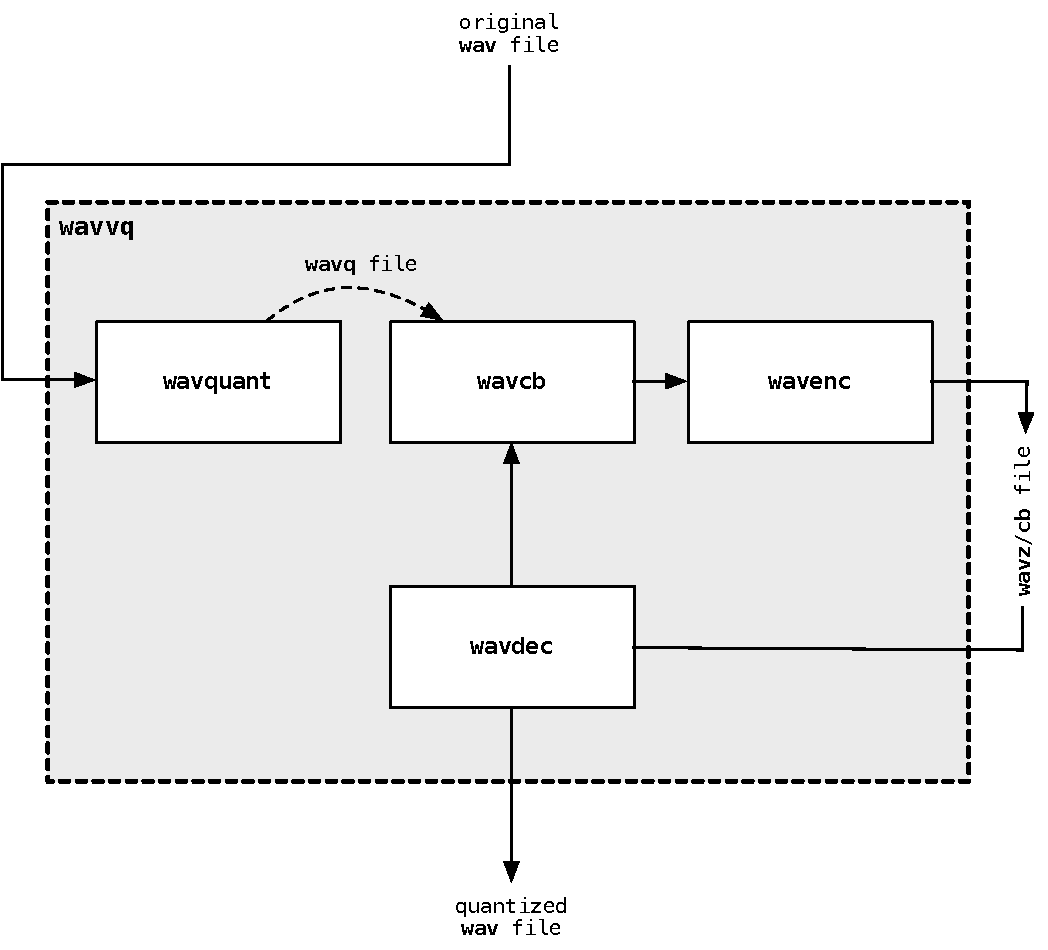
\includegraphics[width=0.45\textwidth]{figs/system-wide-architecture}
	\caption{Lossy audio codec architecture}
    \label{fig:system-wide-architecture}
\end{figure}

%%% THIRD SECTION - Implementation
\section{Implementation}

In this section we deeply describe the implementation of our lossy audio codec.

\subsection{Uniform Quantization}

The first component that we implemented was the \texttt{wavquant} module, since is the first to modify the input audio file given to our system. 

This module receives a \ac{WAV} audio file and an integer quantization factor, $\theta$. Reading each sample $s$ from each frame of the audio file, a new audio file will be created after applying a logical shift operation to each $s$, by a factor of $\theta$, removing the $\theta$ least significant bits. Basically, considering that we have an 8-bits sample $11011010$, by applying a factor $\theta$ of 3 we would get $11011010$ srl $3 = 11011$.

As we want that this module to generate an audio file as output, it is important to have the new samples similar in length to the originals. That is, before saving our changes in a new \ac{WAV} file, it is important to apply the opposite logical shift operation, to revert the length changes and to get the original sample length. Then, this time, we will have a new sample $s'$ which will be the first operation applied with the same operation, in reverse, resulting in the following: $s'=(s$ srl $\theta)$ sll $\theta$.

The output file is then a \ac{WAV} audio file which we called, for simplification purposes, a \texttt{wavq} file and, by this execution, it will still have the same size as the original \texttt{wav} file, since, in length, nothing has changed—only the contents were reduced.

\subsection{Codebook}

The codebook is, by far, the most complex entity created in this project. In fact, this entity must be able to receive instructions on how to construct a codebook and then apply an algorithm to generate the proper number of iterations to enhance its utility.

A general description of the implementation of the codebook (as is in \texttt{wavcb} module) is described as follows in algorithm, where we try to construct a codebook $C$ with $c$ codewords of $b$ bits, with an overlap factor $\alpha$ and a maximum wanted distortion between iterations $\varepsilon$:

\begin{algorithmic}[1]
	\REQUIRE $c > 0$ \AND $b > 0$ \AND $\alpha > 0$ \AND $\varepsilon$
	\STATE \scshape{GenerateCentroids()}
	\STATE $iteration \leftarrow 0$ \COMMENT{\upshape{the current iteration}}
	\STATE $lastDist \leftarrow \infty$ \COMMENT{\upshape{the distortion between iterations}}
	\WHILE{$\neg$\scshape{HasConverged()} \upshape \OR $\neg$\scshape{IsMaxIter()}\upshape}
		\STATE \scshape{TestSamplesOnCentroids()}\upshape
		\STATE $dist \leftarrow$ \scshape{EvaluateDistortion()}\upshape
		\IF{$lastDist - dist < \varepsilon$}
			\STATE $C \leftarrow centroids$
			\STATE \scshape{MarkHasConvergedAs(}\upshape\TRUE{\scshape{)}\upshape}
		\ENDIF
		\STATE $lastDist \leftarrow dist$
		\STATE \scshape{EvaluateNewCentroids()}\upshape
		\STATE $iteration \leftarrow iteration + 1$
	\ENDWHILE
\end{algorithmic}

Looking to the described algorithm we can verify that the first task we do is a method named \scshape{GenerateCentroids()}\upshape. This method is our codebook initialization, which will use the audio file loaded in time of the construction of an object \scshape{Codebook}\upshape, where the algorithm above forms a \scshape{CreateCodebook()} \upshape method. This generation is made according to the algorithm that follows, where $cent$ is the vector of centroids:

\begin{algorithmic}[1]
	\REQUIRE $s$ as samples \AND $c > 0$ \AND $b > 0$ \AND $\alpha > 0$
	\FOR{$i=0$ \TO \scshape size($s$)\upshape $\times b - b$}
		\STATE $cent$.\scshape add($s$($i/16$) \upshape sll ($i$ mod $b$) \OR \scshape add(($s$($i/16$)+1) \upshape srl (b-($i$ mod $b$))
		\STATE $cent \leftarrow$ \scshape DeleteDuplicates($cent$) \upshape 
		\IF{\scshape size($cent$) $< c$\upshape}
			\RETURN error
		\ENDIF
		\STATE $cent \leftarrow$ \scshape ChooseCVectors($cent$, $c$) \upshape
	\ENDFOR
\end{algorithmic}

After executing the \scshape GenerateCentroids() \upshape method we have a vector of $c$ $b$-bit bit sequences which forms our initial set of centroids to test out our training set. 

Now, by considering our samples $s$ as our training set, we try to apply the \ac{LBG} algorithm (also known as generalized Lloyd's algorithm and similar to data clustering's K-means technique), we can, iteration-by-iteration, obtain a good codebook, that is, such a structure that would give us the best set of representations to our audio samples, with which, after the process of decoding, the audio would be the closest possible against the original version.

This algorithm is then expressed on the execution of the \scshape TestSamplesOnCentroids() \upshape method, shown as follows:

\begin{algorithmic}[1]
	\REQUIRE $s$ as audio samples \AND $cent$ as centroids 
	\FORALL{$sample$ in $s$}
		\STATE $\delta = \infty$ \COMMENT{distance}
		\STATE $\delta^\star = \infty$ \COMMENT{temporary distance}
		\STATE $\omega \leftarrow 0$ \COMMENT{minimum distance centroid index}
		\FOR{$i=0$ \TO $cent.$\scshape{size()}\upshape}
			\STATE $\delta^\star \leftarrow$ \scshape{Distance($sample$,$cent(i)$)} \upshape
			\IF{$\delta^\star < \delta$} 
				\STATE $\delta = \delta^\star$
				\STATE $\omega = i$
			\ENDIF
		\ENDFOR
		\STATE $samples_{it}\left[\omega\right].$\scshape{add($(sample,\delta)$)}\upshape
	\ENDFOR
\end{algorithmic}

In the algorithm above there are two items which deserve a little more explanation. Starting by the method \scshape{Distance()}\upshape, this is a method to estimate the euclidean distance between points of dimension $b$. The other item which requires some attention is the structure where we are saving all our results from the LBG method's execution: the $samples_{it}$ vector. This structure is a vector with the size of the $cent$ vector, in which each index has its own vector of tuples, each representing the tested sample and its estimated distance to the corresponding and chosen centroid.

Right after the audio sample training set testing on the centroids which were created we should analyze the quality of the iteration results. To do so, one should estimate the distortion of the current iteration. This is the meaning of the \scshape{EvaluateDistortion()} \upshape method, described below:

\begin{algorithmic}[1]
	\REQUIRE $s_{it}$ as the iteration result \AND $n$ samples count
	\STATE $sum \leftarrow 0$
	\FORALL{$centroid$ in $s_{it}$} 
		\FORALL{$sample$ in $centroid$}
			\STATE $sum \leftarrow sum + sample(1)$
		\ENDFOR
	\ENDFOR
	\RETURN $sum/n$
\end{algorithmic}

Having estimated the distortion, then we only need to calculate the new set of centroids, in order to repeat our algorithm and make a step towards the convergence of the codebook, as we want to. Then, we execute the method \scshape{EvaluateNewCentroids()}\upshape, detailed in the algorithm below:

\begin{algorithmic}[1]
	\REQUIRE $s_{it}$ as the iteration result
	\FORALL{$centroid$ in $s_{it}$}
		\STATE $point \leftarrow $\scshape{GetAverageCentroid($centroid$)}\upshape
		\STATE $centroids.\left[centroid\right]=point$
	\ENDFOR
\end{algorithmic}

Our codebook implementation also relies on a set of other functions such as \scshape{Codebook.Save()} \upshape and \scshape{Codebook.Load()}\upshape. These functions save and load a \texttt{*.cb} file which contains, in binary, the contents of the codebook—the codewords, in a contiguous sequence.

\subsection{Encoder and Decoder}

As soon as the codebook is created by the \texttt{wavcb} module, the task of giving a sample to test on it is a responsibility of an encoder. Then to reverse the process one should use a decoder. 

In our implementation, the encoder is described on the \texttt{wavenc} module. This class \scshape{Encoder} \upshape receives, in order to construct such an object, a codebook, an audio file to compress and a file name to give as an output. This output, then, will be a compressed file with unreadable audio, by a conventional media player, since it will be made with the indexes of the codewords which the codebook gave away, after testing each audio sample with a closest vector within itself.

More than the compressed audio samples themselves, the encoder also has the duty of filling a header with the specifications of such audio file. Without it, the decoder would be blind and could not fulfill to create a new audio file without information such as the format, the sample rate or the number of channels, in a generalized solution.

The decoder, then, specified by the class \scshape{Decoder} \upshape present on the module \texttt{wavdec}, allows us to construct such an object via a file name of a compressed audio file and the respective codebook file.

As the decoder receives a compressed audio file name, it tries to open the file and reads its header, saving useful information about how does the final audio file will look like, as its format, its number of channels and its sample rate. Right after such action, the decoder will start the process of giving its records to the codebook, testing them to get the respective vectors, which will conclude on the production of a \ac{WAV} audio file, decompressed.

\subsection{Developed tools for evaluation}

The system's output \ac{WAV} file, in comparison to the first one (the original one) should have its content audible but with less sound quality, that is, with a certain amount of noise added to it. This is justifiable due to the quantization processes made in both uniform and vectorized steps. To proof this, we created two tools which allows us to evaluate the compression made. 

The first tool, an \emph{\ac{WAV} histogram viewer}, shows us the number of times each sample appear in each audio channel, of a given audio file. More, it can also give the histogram of a mono channel made out of the average samples between the two available channels in such \ac{WAV} audio files.

The second tool, a \emph{Signal-to-Noise ratio} estimator, was created to compare two \ac{WAV} audio files—the first being the natural signal (in other words, the original audio file, which we will use to compare to) and the second being the noisy signal (or the compressed audio file). 

Signal-to-Noise ratio means that we want to get a ratio of a desired signal to the level of background noise, in \acp{dB}. To estimate this, $\text{SNR}_\text{dB}$, we must calculate $$\text{SNR}_\text{dB}=10\log_{10}{\frac{P_{\text{signal}}}{P_{\text{noise}}}}$$, where $P_{\text{signal}}$ is the power of the [original] signal and $P_{\text{noise}}$ is the power of the background noise.

Given such information, comparing two equal files must be theoretically infinity, what gives us the conclusion that the bigger the value, the better the compressed audio file is.

In order to calculate the power of a signal we applied the following algorithm, where $S$ is a vector of the original samples and $M$ is the vector of the compressed audio samples, after decoding:

\begin{algorithmic}[1]
	\REQUIRE $S$ as original samples \AND $M$ as modified samples
	\STATE $\text{sum}_{\text{original}} \leftarrow 0$
	\FORALL{$\text{value}$ in $S$}
		\STATE $\text{sum}_{\text{original}} \leftarrow \text{sum}_{\text{original}} + \text{value}\times \text{value}$
	\ENDFOR
	\STATE $\text{sum}_{\text{modified}} \leftarrow 0$	
	\FOR{$i=0$ \TO $S.$\scshape{size()}\upshape}
		\STATE $\text{sum}_{\text{modified}} \leftarrow \text{sum}_{\text{modified}}+\left(S\left[i\right] - M\left[i\right]\right)^2$
	\ENDFOR
	\RETURN $10\times\log_{10}{\left(\text{sum}_{\text{original}}/\text{sum}_{\text{modified}}\right)}$
\end{algorithmic}

%%% FOURTH SECTION - Evaluation
\section{Evaluation}

As our implementations produced some results, in this section we establish an analysis of them.

\subsection{Evaluation tools}

Our developed tools to evaluate the lossy audio codec provided meaningful results. Starting by the \ac{WAV} audio histogram plotter, this tool is able to provide us plots on the count of samples per channel on an audio sample set and the average channel histogram as equal.

In the figure~\ref{fig:sample-hist} we can verify the histogram of left, right and mono channels of the sample audio file given by the class' teachers—file \texttt{sample.wav}. 

\begin{figure}
	\centering
	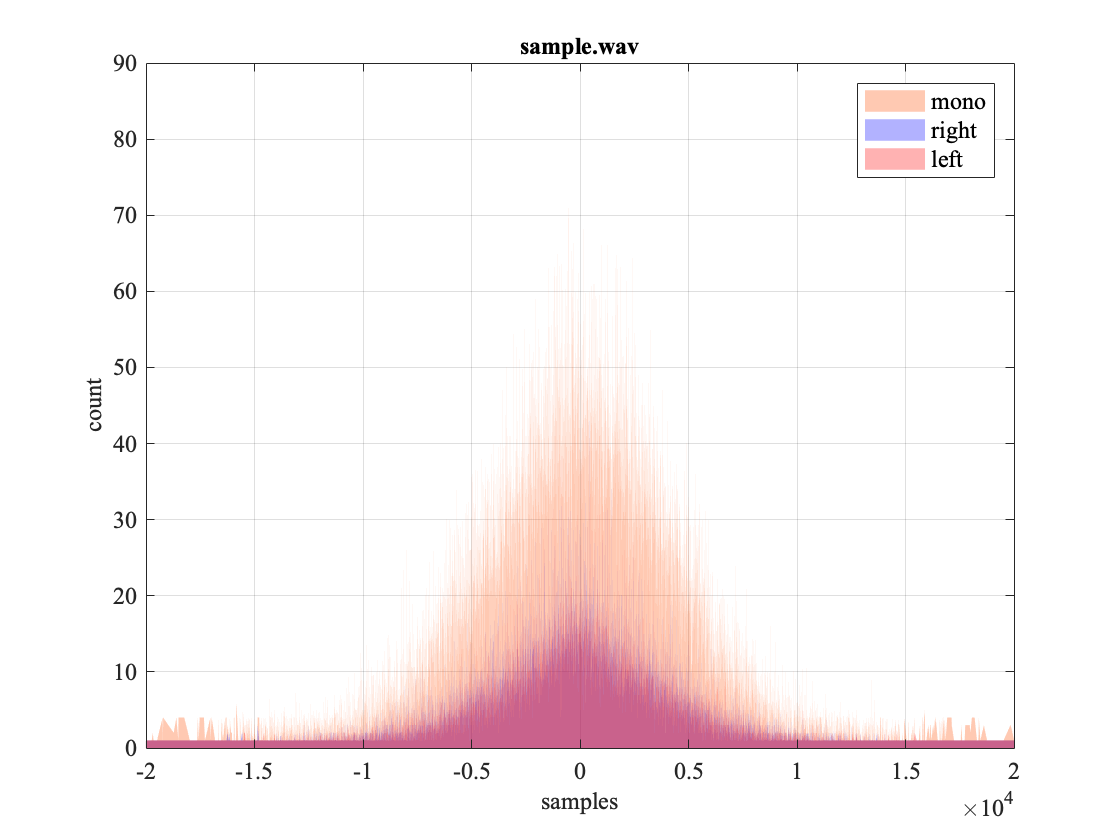
\includegraphics[width=0.5\textwidth]{figs/original-hist.png}
	\caption{Left, right and mono channels histogram (\texttt{sample.wav}, 16-bit audio)}
    \label{fig:sample-hist}
\end{figure}

As we can analyze from the figure~\ref{fig:sample-hist} while both left and right channel's samples are quite similar in terms of number of appearances on the audio file, when we produce the average channel, more samples appear equal, since the probability of being so is almost the double than before.

In terms of our other tool—the Signal-to-Noise ratio estimator—this also gives useful results, as expected by its theoretical development. When we presented its implementation, we stated that if two equal audio files are submitted into such a comparison, then a value of infinity should arise. In fact, in our implementation, when we do so, the IEEE 754 value of \texttt{inf} is printed as output. 

\subsection{Uniform quantization}

If we apply uniform quantization to our \texttt{sample.wav} file, then we should verify that both left and right channels appear more often with the same samples, as we just decreased the size of the possible combinations of samples in this audio. In figure~\ref{fig:sample-5-hist} such a scenario is possible to be proofed, where we produced a quantization of 5 bits.

\begin{figure}
	\centering
	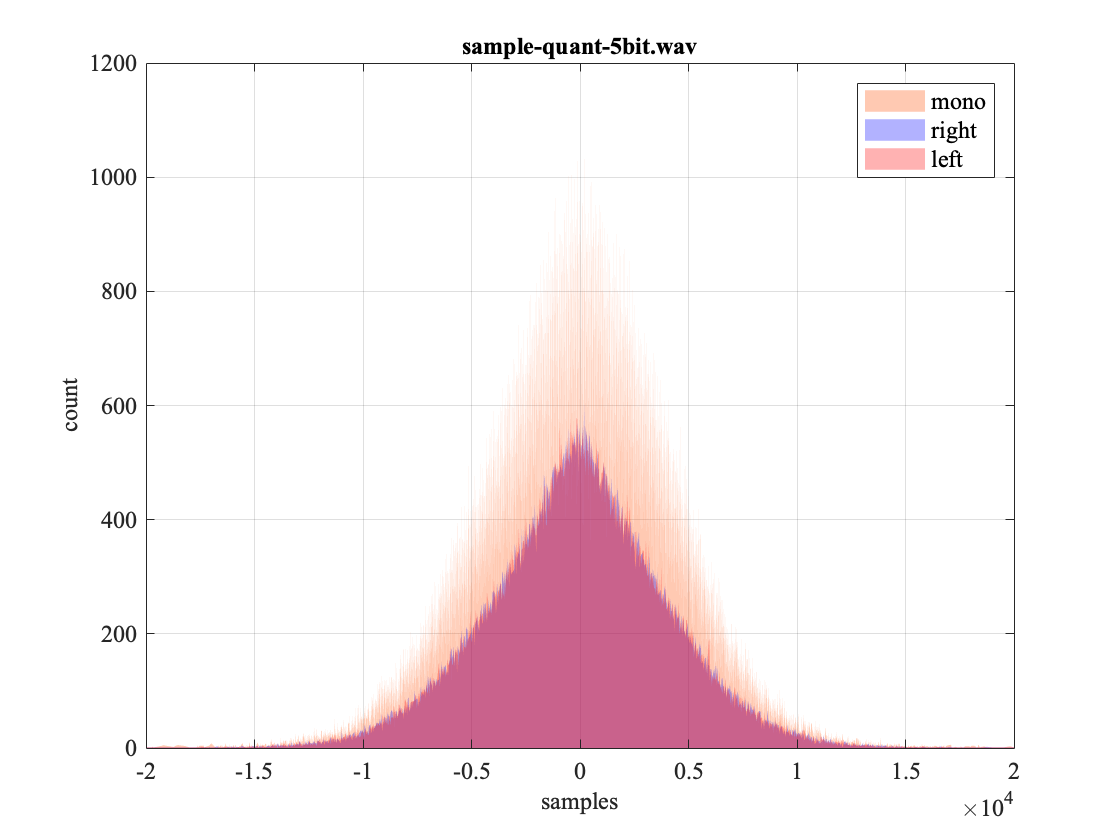
\includegraphics[width=0.5\textwidth]{figs/5-hist.png}
	\caption{Left, right and mono channels histogram (\texttt{sample.wav}, 16-bit audio quantized in 5 bits)}
    \label{fig:sample-5-hist}
\end{figure}

As we obtained, by hearing, the maximum quantization in which this file is submitted, maintaining useful information for us humans, is of 10 bits. In figure~\ref{fig:sample-10-hist} is depicted such a set of histograms.

\begin{figure}
	\centering
	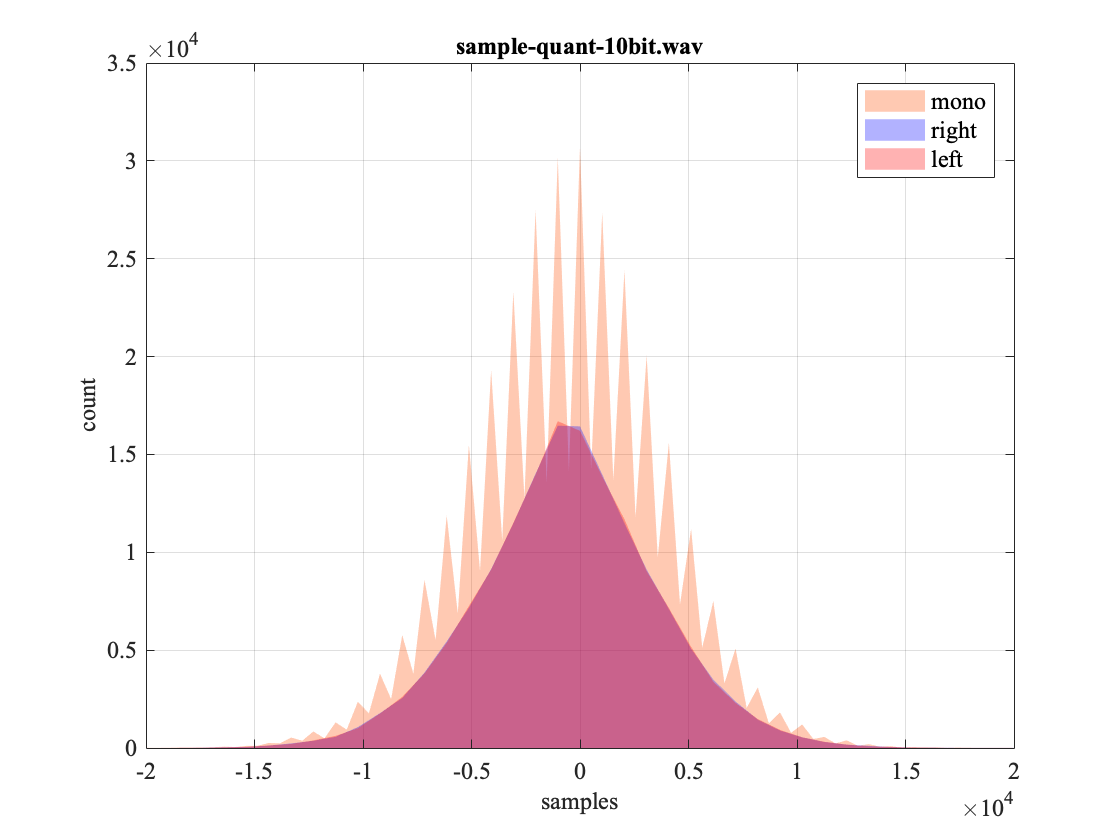
\includegraphics[width=0.5\textwidth]{figs/10-hist.png}
	\caption{Left, right and mono channels histogram (\texttt{sample.wav}, 16-bit audio quantized in 10 bits)}
    \label{fig:sample-10-hist}
\end{figure}

In the figure~\ref{fig:sample-10-hist}, in fact, is very clear to see that as we just decreased our range of representation of each sample to just 6 bits, our average channel starts to show its discrete values easily—the values have always been discrete, but the histogram resolution did not allows us to see it.

If we increase even more, the quantization (to 14 bits, i.e.) we can see that the histogram is heavily saturated, with which we can, by itself, guess that the audio would be completely inaudible (figure~\ref{fig:sample-14-hist}).

\begin{figure}
	\centering
	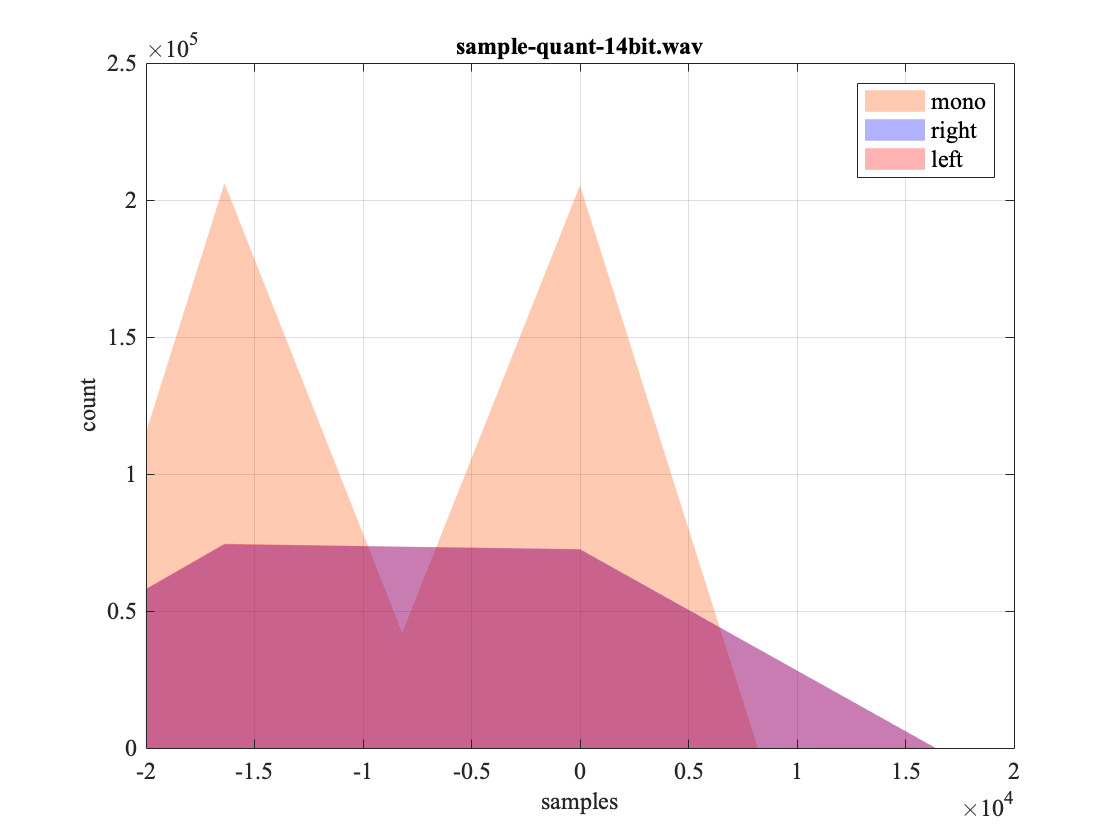
\includegraphics[width=0.5\textwidth]{figs/14-hist.png}
	\caption{Left, right and mono channels histogram (\texttt{sample.wav}, 16-bit audio quantized in 14 bits)}
    \label{fig:sample-14-hist}
\end{figure}

In terms of Signal-to-Noise ratio, the following results were obtained, as we can see in table~\ref{tab:table}.

\begin{table}[!t]
\renewcommand{\arraystretch}{1.3}
\caption{Signal-to-Noise Ratio by Quantization Factor}
\label{tab:table}
\centering
\begin{tabular}{c||c}
\hline
\textbf{Quantization} & \textbf{SNR} \\ 
\hline\hline
0 & $\infty$ dB \\
2 & 66.8418 dB \\
4 & 53.3973 dB \\
6 & 41.0444 dB \\
8 & 28.9237 dB \\
10 & 16.8549 dB \\
12 & 4.77507 dB \\
14 & -7.70631 dB \\
15 & -14.3015 dB \\
16 & 0 dB \\ 
\hline
\end{tabular}
\end{table}

As we can see by the results, it is proved that the closer the SNR is to infinity, the better the sound quality is, since the quantization factor is smaller. We can also notice that if the quantization is maximum, then the value will be closer to 0 dB.

\subsection{Vector quantization}

Unfortunately, we could not produce any result with vector quantization at the time of this work delivery. This happened because of the implementation of the codebook, which did not let us test its unit in such a short time after we have completed it.

%%% FIFTH SECTION - Conclusions
\section{Conclusions}

This work not only has showed us the effects of lossy compression on an audio file, but also gave us the comprehension we needed in terms of analysis of its histograms to better understand the effects on the quantity range of representation of each sample present on an audio file.

While we have learned a large number of concepts, misfortunately we could not attend the delivery deadline with a complete work, letting such a space for fixing the codebook issues and to implement some other features.

If this work had already been done, one could study some different strategies of implementing codebooks, with different algorithms, basing its initialization on different features, such as the average sample of a given file to compress or other. Moreover, one could also juxtapose both encoded file and codebook and create one media player which would be able to read the media.

%%% SIXTH SECTION - Group Collaboration Assessment
\section{Group Collaboration Assessment}

After some deliberation within the work group we have decided to distribute the working time by each member in the following percentages: 

\begin{itemize}
	\item João Fonseca — 10\% of total time;
	\item Pedro Silva — 10\% of total time;
	\item Rui Lopes — 80\% of total time.
\end{itemize}

\end{document}

%%%%% DOCUMENT END